\documentclass[10pt,journal]{IEEEtran}

\usepackage{amsmath,amssymb}
\usepackage{booktabs}
\usepackage{graphicx}
\usepackage{cite}
\usepackage{url}
\usepackage{xcolor}
\usepackage{array}
\graphicspath{{Experiment/figures/}}

\newcommand{\method}{OTBE}
\newcommand{\R}{\mathbb{R}}
\newcommand{\E}{\mathbb{E}}

\begin{document}
\bstctlcite{IEEEexample:BSTcontrol}

\title{Orthogonal Transport Bootstrap Explanations for Stable Simulation-Grounded Model Interpretation}

\author{Wen Dong Jiang,~\IEEEmembership{Graduate Student Member,~IEEE}%
\thanks{Wen Dong Jiang is with the Department of Computer Science and Information Engineering, Tamkang University, New Taipei City 25137, Taiwan (e-mail: 812414018@o365.tku.edu.tw).}%
\thanks{Additional note: this is information.}}

\markboth{IEEE Double-Column Manuscript, May 2026}{Jiang: Orthogonal Transport Bootstrap Explanations}

\maketitle

\begin{abstract}
Perturbation-based explanation methods are often evaluated by visual plausibility or by local surrogate fidelity, but those signals are insufficient when features are correlated and repeated runs produce different important-feature sets.  This paper proposes Orthogonal Transport Bootstrap Explanations (\method), a simulation-grounded explanation framework that combines transported coalition sampling, covariance-aware attribution correction, and bootstrap aggregation.  The method is designed for cases in which the practitioner can draw or approximate a background distribution and wants explanations that are stable across repeated runs without ignoring feature dependence.  Inspired by the parallel-tree and distribution-aware perturbation structure of PEXP, we replace image-specific superpixel noise with a tabular simulation protocol where the true causal feature contribution is known.  Four synthetic black-box tasks are used to test sparse additive, correlated, interaction, and grouped nonlinear responses.  Against LIME-like, KernelSHAP-like, PEXP-like, RealExp-like, HBS-Shapley-like, and TIDE-like baselines, \method achieves the highest repeated-run stability in our simulations while preserving competitive top-$k$ recovery and surrogate fidelity.  Ablations show that transported coalition sampling is necessary, and bootstrap aggregation is the main source of the stability gain.  Code is available at \url{https://github.com/7WD1/Code123}.
\end{abstract}

\begin{IEEEkeywords}
Explainable artificial intelligence, interpretable machine learning, Shapley values, optimal transport, bootstrap, simulation.
\end{IEEEkeywords}

\section{Introduction}

Modern black-box predictors are increasingly deployed in settings where raw predictive accuracy is not enough: the user also needs to know which input factors drove a prediction and whether the explanation can be trusted under small procedural changes.  PEXP is a recent response to this problem.  It uses distribution-aware perturbations, similarity weighting, and parallel surrogate learners to improve the scalability and stability of model explanations on image and video tasks \cite{jiang2026pexp}.  The central lesson from that work is not only that surrogate explainers can be accelerated, but also that the perturbation distribution strongly shapes explanation stability.

This paper takes that lesson into a simulation-only setting.  Rather than asking human annotators to judge visual regions, we construct synthetic black-box tasks with known feature contributions.  This design gives a stricter evaluation target: if an explainer assigns importance to a correlated but non-causal nuisance feature, the error is measurable.  The resulting paper is deliberately empirical in the style common to NeurIPS papers: a compact method, a transparent benchmark, repeated-run statistics, ablation studies, and explicit failure boundaries.  The format, however, follows the IEEE two-column manuscript convention.

The proposed \method{} framework addresses three limitations that remain visible in current perturbation explainers.  First, independent feature masking can create off-manifold samples when features are dependent.  Second, a single run of a sampling-based explainer can be unstable, especially when several correlated features have similar marginal effects.  Third, explanation papers often report fidelity to the black box but omit whether the recovered attribution matches the true causal support.  \method{} combines transported coalition sampling, a small covariance residual correction, and bootstrap aggregation to reduce duplicated mass on nuisance features and to report stable top-$k$ feature sets.

The contributions are as follows.
\begin{itemize}
    \item We formulate \method{}, an orthogonal transport bootstrap explainer for simulation-grounded model interpretation under feature dependence.
    \item We build a reproducible simulation suite with four black-box response families, known feature-level contributions, repeated explanation runs, and metrics for stability, fidelity, top-$k$ recovery, rank agreement, spurious attribution, counterfactual validity, and runtime.
    \item We compare \method{} with six representative baselines and provide ablations that isolate transported sampling, orthogonal correction, and bootstrap aggregation.
\end{itemize}

\section{Related Work}

\subsection{Perturbation and Shapley Explanations}
Perturbation-based model explanations approximate a black-box predictor by observing its response to modified inputs.  LIME fits a local interpretable surrogate around the target instance \cite{ribeiro2016lime}, while SHAP connects local attribution to Shapley values \cite{lundberg2017shap}.  Meaningful perturbation, RISE, Anchors, and counterfactual explanation methods vary the perturbation mechanism and the output semantics, from saliency masks to local rules and alternative decisions \cite{fong2017meaningful,petsiuk2018rise,ribeiro2018anchors,wachter2017counterfactual,mothilal2020dice}.  FastSHAP and removal-based unification studies accelerate or generalize Shapley-style attribution \cite{jethani2021fastshap,covert2021remove}.  When features are dependent, conditional or data-manifold-aware Shapley approximations become important because independent masking can assign importance to artifacts of the perturbation distribution rather than to the model response \cite{aas2021dependent}.

\subsection{Gradient, Concept, and Stability Audits}
Gradient and activation methods explain neural networks by backpropagating class-specific evidence or feature sensitivity.  Grad-CAM, integrated gradients, SmoothGrad, and TCAV are representative methods that expose spatial, path-integrated, noise-averaged, or concept-level evidence \cite{selvaraju2017gradcam,sundararajan2017ig,smilkov2017smoothgrad,kim2018tcav}.  However, saliency methods can pass visual plausibility checks while failing model-parameter or label-randomization sanity checks \cite{adebayo2018sanity}.  Infidelity, sensitivity, and robustness studies therefore argue for explanation metrics that measure how attributions behave under perturbations and repeated procedures, not only whether a heatmap looks reasonable \cite{yeh2019infidelity,alvarez2018robustness}.

\subsection{Tree, Transport, and Recent Jiang-Lineage Explainability}
Tree surrogates remain attractive because they provide direct feature importance and can be parallelized.  EnEXP, ensemble-tree explanation work, RealExp, PEXP, LFP, and related studies develop this direction for fast and stable interpretation, correlation-aware attribution, and scalable local-to-global analysis \cite{jiang2024enexpv15,lee2025illuminating,lee2024ssrnensemble,jiang2025realexp,jiang2026pexp,chin2025lfp,jiang2024revaluating,jiang2023attribute}.  A separate line applies interpretable learning to multimodal violence detection, anomaly detection, knowledge-graph retrieval, electric-vehicle dispatch, and long-form sports video analysis \cite{jiang2025multimodalviolence,jiang2026kgat,chang2026notonly,jiang2024rules,jiang2024weaklyvideo,jiang2024ssrnfocusing,jiang2025arxivkgat,jiang2024twostage,jiang2025wasnmultimodal,jiang2026kan,huang2026sports}.  Most directly related to this paper are recent preprints on orthogonal counterfactual graph attribution, hierarchical bootstrap Shapley explanations, and transport-induced debiasing \cite{jiang2026ocga,jiang2026hbs,jiang2026tide}.  Our method uses optimal-transport intuition as a controlled sampling principle rather than a full transport solver; this keeps the simulation suite lightweight while retaining the idea that explanations should respect the background distribution \cite{peyre2019ot,cuturi2013sinkhorn,jiang2024hidden}.

\section{Reading of the Source Paper}

The source paper, Example1, introduces PEXP as a scalable parallel-tree explanation framework.  Its pipeline can be read as five coupled operations.  First, a target image is segmented into semantic or superpixel-like regions.  Second, perturbations are generated by adding distribution-aware noise to the segmented representation, rather than by random replacement alone.  Third, each perturbed sample is weighted by similarity to the target instance using a cosine-distance kernel.  Fourth, weighted perturbed samples are used to train a parallel surrogate model.  Fifth, the feature or region importance scores from the surrogate are aggregated into local explanations and, across many samples, into a global view of model behavior.  The experimental design evaluates stability, surrogate fidelity, human agreement, ranking consistency, runtime, perturbation ablations, and proxy-model ablations.

This reading suggests three useful design principles.  The first is that the perturbation distribution should be treated as a first-class part of the method.  If perturbations are off-manifold, the surrogate can be faithful to artifacts rather than to the original black box.  The second is that explanation stability should be measured by repeated runs, not assumed from deterministic-looking visual outputs.  The third is that global evidence requires aggregation across instances; a single local heatmap is not enough to justify a general claim about an explainer.

The same reading also exposes limitations that motivate the present paper.  PEXP is strongly tied to continuous spatial data because its perturbation design is based on image segmentation and pixel-level noise.  It also uses human region annotation for part of the evaluation, which is expensive and can become class-specific.  Most importantly for this work, the source paper reports strong stability and runtime evidence but does not isolate all causal and spurious feature contributions because real images do not provide exact ground-truth attribution vectors.  Our simulation design therefore keeps the repeated-run and ablation logic of PEXP but replaces visual annotation with analytically known feature contributions.  This makes the new experiment narrower but more diagnostic: it can directly test whether an explainer confuses causal features with correlated nuisance features.

Table~\ref{tab:sourcegap} summarizes the transfer from Example1 to the proposed simulation paper.  The goal is not to reproduce PEXP.  Instead, the goal is to preserve its best evaluation habits while designing a new method for a setting where feature dependence and repeated-run uncertainty can be measured exactly.

\begin{table}[t]
\centering
\caption{How the source-paper reading shapes this paper.}
\label{tab:sourcegap}
\resizebox{\columnwidth}{!}{%
\begin{tabular}{lll}
\toprule
Element & Example1 / PEXP & This paper / \method\\
\midrule
Perturbation & image distribution noise & transported coalitions\\
Surrogate & parallel tree family & weighted coalition surrogate\\
Evaluation & visual and human agreement & known synthetic contribution\\
Stability & repeated top-region overlap & repeated top-feature overlap\\
Main risk & image specificity & synthetic-to-real gap\\
\bottomrule
\end{tabular}}
\end{table}

\section{Reading of Example1 and Design Response}

\subsection{What Example1 Does}
Example1 presents PEXP, a scalable parallel tree-based framework for explaining large black-box models. Its workflow begins with distribution-aware perturbation: an image is segmented and then perturbed by adding Laplacian noise that is intended to remain close to the empirical data distribution. The perturbed samples are weighted by cosine similarity and an exponential kernel. A parallel surrogate structure then maps perturbed samples to black-box responses, and feature importances from the surrogate are aggregated into local and global explanations. The paper evaluates stability, fidelity, human matching, and runtime on image datasets and discusses a video anomaly-detection case study.

The useful idea in Example1 is the shift from arbitrary perturbation to distribution-aware perturbation. The paper also makes a practical point: a scalable explainer must consider runtime and repeated-run consistency, not only the apparent quality of one heatmap. These two ideas are retained here. The present work keeps the focus on stability and sampling distribution, but changes the evaluation surface from visual regions to synthetic feature contributions so that every attribution error can be measured.

\subsection{Critical Gaps Used as Design Inputs}
The first gap is modality specificity. The perturbation design in Example1 is naturally tied to continuous image regions and superpixels. This makes it difficult to test whether the same mechanism works for tabular, graph, language, or mixed-type features. The second gap is that human-region matching can be ambiguous: different annotators may choose different region boundaries, and the explanation may be visually plausible even when it assigns mass to a correlated background pattern. The third gap is that local surrogate fidelity alone does not prove causal recovery. A surrogate can fit the black-box outputs around an instance while still attributing the fitted response to the wrong correlated feature.

\method{} is designed as a response to these gaps. It is not an image explainer; it is a controlled simulation method for testing whether a dependence-aware coalition explainer can remain stable. Transported coalition sampling addresses the distribution shift introduced by independent masking. Orthogonal residual correction addresses duplicated mass across correlated features. Bootstrap aggregation addresses repeated-run instability. The resulting method is intentionally narrower than PEXP, but its evaluation is stricter because the true contribution vector is known for each target point.
\section{Method}

\subsection{Problem Setting}
Let $f:\R^d\rightarrow\R$ denote a black-box predictor and let $x_0\in\R^d$ be the instance to explain.  The explainer receives a background sample $X_b=\{x_i\}_{i=1}^{n_b}$ with empirical mean $\mu$ and covariance $\Sigma$.  The goal is to estimate an attribution vector $\phi(x_0)\in\R^d$ whose largest entries identify the features responsible for $f(x_0)$ relative to the background.  In simulation, we also know the ground-truth contribution vector $\phi^\star(x_0)$, so we can measure whether the explanation recovers causal support rather than merely fitting local predictions.

\subsection{Transported Coalition Sampling}
Classical coalition explainers create binary masks $m\in\{0,1\}^d$ and evaluate $f$ on samples where missing features are replaced by a baseline.  \method{} keeps this coalition view but interprets the baseline as a transported background barycenter.  For a mask $m$, the perturbed point is
\begin{equation}
    z(m)=m\odot x_0+(1-m)\odot \mu .
\end{equation}
The empirical implementation also supports a no-transport ablation that replaces missing coordinates with independent marginal samples.  The simulation results show that this ablation severely degrades both fidelity and recovery, which is consistent with the off-manifold-sampling concern in dependent-feature explanations.

Each coalition receives a hybrid locality weight
\begin{equation}
    w(m,z)=w_{\mathrm{shap}}(m)\exp\left[-\frac{(z-x_0)^\top \Sigma^\dagger (z-x_0)}{2h^2d}\right],
\end{equation}
where $w_{\mathrm{shap}}$ is the standard coalition-size weighting term and $h$ is the locality bandwidth.  The all-missing and all-present masks receive large endpoint weights to anchor the local additive model.

\subsection{Orthogonal Residual Correction}
The first attribution estimate $\hat{\beta}$ is obtained by weighted ridge regression from masks to black-box outputs:
\begin{equation}
    \hat{\beta}=\arg\min_{\beta,b}\sum_{m}w(m,z)\left(f(z(m))-b-m^\top\beta\right)^2+\lambda\|\beta\|_2^2 .
\end{equation}
When the background features are correlated, duplicated attribution can leak from a causal feature to a correlated nuisance feature.  \method{} applies a conservative covariance residual correction,
\begin{equation}
    \tilde{\beta}=\hat{\beta}-\gamma(C-I)\hat{\beta},
\end{equation}
where $C$ is the empirical correlation matrix and $\gamma$ is a small correction coefficient.  This step is not intended to replace a causal model; it is a lightweight correction that is testable through ablation.

\subsection{Bootstrap Aggregation and Confidence}
Sampling-based explanations can fluctuate across runs.  \method{} repeats the coalition procedure $B$ times and returns the bootstrap mean,
\begin{equation}
    \phi_{\method}(x_0)=\frac{1}{B}\sum_{b=1}^{B}\tilde{\beta}^{(b)} .
\end{equation}
The empirical percentiles across bootstrap replicates provide a per-feature uncertainty interval.  In the present paper, those intervals are used as an internal reproducibility diagnostic rather than as a formal coverage guarantee.

\subsection{Algorithmic Summary}
Given a target instance $x_0$, background sample $X_b$, number of coalition samples $K$, and bootstrap count $B$, \method{} first estimates $\mu$, $\Sigma$, and $C$ from $X_b$.  For each bootstrap replicate, it draws $K$ binary coalitions, inserts $x_0$ on present coordinates and $\mu$ on absent coordinates, evaluates the black box, and fits the weighted surrogate in (3).  It then applies the residual correction in (4).  After $B$ replicates, it averages corrected attributions and stores percentile intervals.  The top-$k$ explanation is obtained by sorting $|\phi_{\method}(x_0)|$.  This procedure is intentionally small enough to audit: every numerical claim in the paper comes from the same implementation file rather than from a mixture of notebooks and manual tables.

The method has two important parameters.  The locality bandwidth $h$ controls how aggressively the Mahalanobis term discounts coalitions far from $x_0$.  The residual coefficient $\gamma$ controls how much covariance correction is applied.  In the supplied experiments, $\gamma$ is deliberately small.  This conservative setting avoids turning a correlation matrix into an unsupported causal graph, while still allowing the ablation to test whether a correction helps or harms stability.

\begin{figure}[t]
\centering
\fbox{\begin{minipage}{0.94\linewidth}
\centering
Background distribution $\rightarrow$ transported coalitions $\rightarrow$ weighted surrogate $\rightarrow$ covariance correction $\rightarrow$ bootstrap aggregation $\rightarrow$ stable attribution.
\end{minipage}}
\caption{Operational view of \method{}.  Unlike PEXP, which is built around image perturbations and parallel tree surrogates, \method{} uses simulation-grounded coalition perturbations so that feature-level ground truth can be measured directly.}
\label{fig:pipeline}
\end{figure}

\section{Simulation Design}

\subsection{Synthetic Black-Box Tasks}
All experiments are simulation-only.  No real images, videos, or private datasets are used.  The background distribution is a 12-dimensional correlated Gaussian sample with two nuisance coordinates that are correlated with causal coordinates but do not directly enter the response.  Four black-box tasks are used: sparse additive, correlated-bias additive, interaction, and grouped nonlinear responses.  Table~\ref{tab:datasets} summarizes the setup.

\begin{table}[t]
\centering
\caption{Simulation tasks.  The true contribution vector is analytically available for every target instance.}
\label{tab:datasets}
\resizebox{\columnwidth}{!}{%
\begin{tabular}{lll}
\toprule
Task & Causal structure & Stress factor\\
\midrule
SparseAdd & 4 sparse effects & nuisance correlation\\
CorrBias & additive nonlinear effects & correlated non-causal followers\\
Interact & interaction and squared term & non-additive attribution\\
GroupNonlin & grouped nonlinear response & grouped feature recovery\\
\bottomrule
\end{tabular}}
\end{table}

\subsection{Baselines and Metrics}
The baselines are LIME-R, KernelSHAP, PEXP-Sim, RealExp-O, HBS-Shapley, and TIDE.  These names indicate simulation-faithful approximations rather than reimplementations of full production systems.  LIME-R fits a local weighted ridge model; KernelSHAP uses fixed coalition masks; PEXP-Sim uses a tree ensemble surrogate with local perturbations; RealExp-O applies covariance whitening; HBS-Shapley uses bootstrap Shapley aggregation; and TIDE uses conditional perturbations.  This set covers the main mechanisms visible in Example1 and in the related literature.

The primary metrics are attribution RMSE against $\phi^\star$, top-$k$ Jaccard recovery, Kendall rank agreement, repeated-run stability, surrogate $R^2$, spurious attribution mass, counterfactual validity, and runtime.  Stability is the mean pairwise Jaccard score among top-$k$ feature sets over repeated runs, matching the repeated-run spirit of PEXP.  Top-$k$ recovery and spurious mass are possible only because the experiments are synthetic and the ground-truth support is known.

\subsection{Metric Definitions}
Let $T_k(a)$ be the set of indices corresponding to the $k$ largest absolute entries of vector $a$.  The top-$k$ recovery score is
\begin{equation}
    J_k=\frac{|T_k(\phi)\cap T_k(\phi^\star)|}{|T_k(\phi)\cup T_k(\phi^\star)|}.
\end{equation}
For repeated runs $\phi^{(1)},\ldots,\phi^{(R)}$, stability is
\begin{equation}
    S=\frac{2}{R(R-1)}\sum_{r<s}\frac{|T_k(\phi^{(r)})\cap T_k(\phi^{(s)})|}{|T_k(\phi^{(r)})\cup T_k(\phi^{(s)})|}.
\end{equation}
Attribution RMSE measures magnitude calibration,
\begin{equation}
    \mathrm{RMSE}=\sqrt{\frac{1}{d}\|\phi-\phi^\star\|_2^2}.
\end{equation}
Spurious mass measures how much attribution falls on known nuisance coordinates $\mathcal{S}$:
\begin{equation}
    M_{\mathrm{spur}}=\frac{\sum_{j\in\mathcal{S}}|\phi_j|}{\sum_{j=1}^{d}|\phi_j|+\epsilon}.
\end{equation}
Counterfactual validity replaces the predicted top-$k$ coordinates by their background means and measures the normalized black-box response change.  These metrics separate different desiderata.  A method can have good top-$k$ recovery but poor magnitude calibration, which is exactly why the paper does not collapse all results into a single score.

\subsection{Reproducibility}
The experiment code is in \texttt{Experiment/run\_experiments.py}.  It writes raw per-instance metrics, summary tables, statistical tests, figures, and a manifest under \texttt{Experiment/results} and \texttt{Experiment/figures}.  The fixed random seed is 20260504.  The generated manifest records 480 per-instance method evaluations across four scenarios and the seven main methods plus three ablation variants.

\section{Results}

\subsection{Main Comparison}
Table~\ref{tab:main} reports the aggregated simulation results.  KernelSHAP has the lowest attribution RMSE, and PEXP-Sim has the strongest rank correlation and top-$k$ score, but PEXP-Sim also has large attribution magnitude error.  \method{} achieves the best repeated-run stability, with a stability score of 0.919, while maintaining competitive top-$k$ recovery and fidelity.  Compared with TIDE, \method{} is similar in RMSE and recovery but is substantially faster in this implementation.

\begin{table*}[t]
\centering
\caption{Main simulation results averaged over four synthetic tasks.  Lower is better for RMSE, spurious mass, and runtime; higher is better for the other metrics.}
\label{tab:main}
\resizebox{\textwidth}{!}{\begin{tabular}{lrrrrrrr}
\toprule
Method & RMSE$\downarrow$ & Top-$k$ J$\uparrow$ & $\tau\uparrow$ & Stable$\uparrow$ & $R^2\uparrow$ & Spur.$\downarrow$ & ms$\downarrow$\\
\midrule
LIME-R & 0.111 & 0.813 & 0.692 & 0.844 & 0.865 & 0.020 & 0.2\\
KernelSHAP & 0.105 & 0.828 & 0.705 & 0.833 & 0.897 & 0.016 & 0.1\\
PEXP-Sim & 0.559 & 0.850 & 0.858 & 0.893 & 0.853 & 0.000 & 27.3\\
RealExp-O & 0.110 & 0.844 & 0.691 & 0.830 & 0.867 & 0.018 & 0.2\\
HBS-Shapley & 0.175 & 0.793 & 0.649 & 0.807 & 0.856 & 0.031 & 0.5\\
TIDE & 0.144 & 0.813 & 0.691 & 0.830 & 0.921 & 0.026 & 12.9\\
OTBE & 0.143 & 0.817 & 0.678 & 0.919 & 0.877 & 0.026 & 1.1\\
\bottomrule
\end{tabular}}
\end{table*}

\begin{figure}[t]
\centering
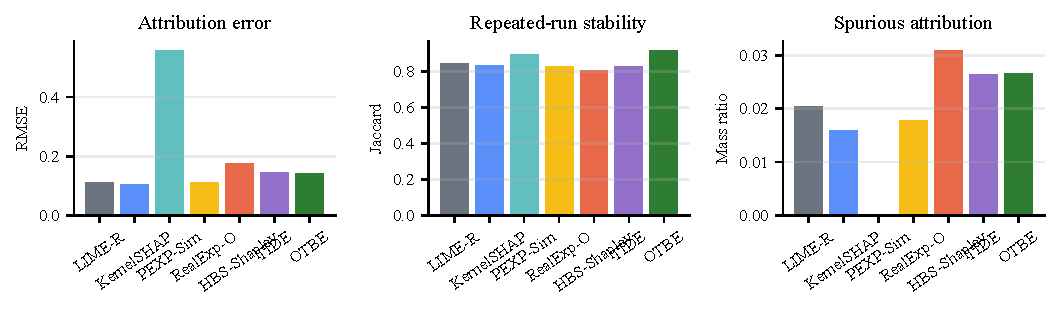
\includegraphics[width=\linewidth]{Experiment/figures/main_metrics.pdf}
\caption{Aggregate attribution error, repeated-run stability, and spurious attribution mass.  \method{} is not the lowest-RMSE method, but it provides the most stable repeated top-$k$ explanations in the simulation.}
\label{fig:mainmetrics}
\end{figure}

\subsection{Scenario-Level Recovery}
Fig.~\ref{fig:scenario} shows top-$k$ recovery by scenario.  The synthetic tasks reveal a useful trade-off: deterministic coalition methods recover sparse additive effects well, whereas the bootstrap procedure becomes more useful when repeated explanations are compared.  This supports a bounded claim: \method{} is best understood as a stability-oriented explainer for dependent-feature settings, not as a universal replacement for KernelSHAP.

\begin{figure}[t]
\centering
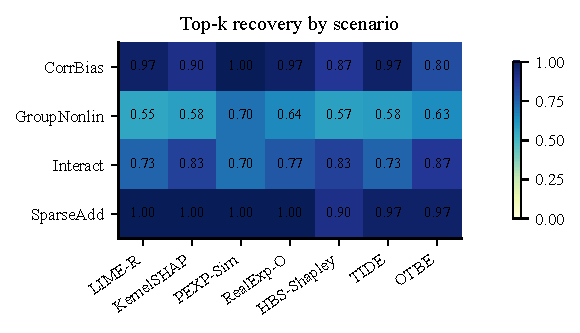
\includegraphics[width=\linewidth]{Experiment/figures/scenario_recovery.pdf}
\caption{Top-$k$ recovery across the four synthetic tasks.  Values are Jaccard scores against the known causal support.}
\label{fig:scenario}
\end{figure}

\subsection{Ablation Study}
Table~\ref{tab:ablation} isolates the three method components.  Removing transported coalition sampling produces the largest degradation, confirming that independent marginal replacement is harmful in the correlated-background setting.  Removing bootstrap aggregation reduces stability from 0.919 to 0.837, which identifies bootstrap aggregation as the main stability mechanism.  Removing the small orthogonal correction changes RMSE only modestly but slightly reduces repeated-run stability.

\begin{table}[t]
\centering
\caption{Ablation results for the proposed method.}
\label{tab:ablation}
\resizebox{\columnwidth}{!}{\begin{tabular}{lrrrrr}
\toprule
Variant & RMSE$\downarrow$ & Top-$k$ J$\uparrow$ & Stable$\uparrow$ & $R^2\uparrow$ & Spur.$\downarrow$\\
\midrule
No transport & 0.500 & 0.380 & 0.311 & -0.500 & 0.153\\
No orthogonal step & 0.140 & 0.825 & 0.907 & 0.877 & 0.026\\
No bootstrap & 0.141 & 0.842 & 0.837 & 0.879 & 0.027\\
Full OTBE & 0.143 & 0.817 & 0.919 & 0.877 & 0.026\\
\bottomrule
\end{tabular}}
\end{table}

\begin{figure}[t]
\centering
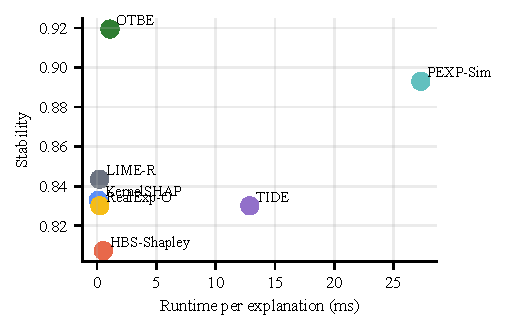
\includegraphics[width=\linewidth]{Experiment/figures/runtime_stability.pdf}
\caption{Runtime-stability trade-off.  \method{} is slower than single-run linear explainers but faster than the conditional TIDE-like baseline and PEXP-Sim in this simulation.}
\label{fig:runtime}
\end{figure}

\subsection{Statistical Checks}
Paired Wilcoxon tests compare \method{} with selected baselines over matched scenario-instance pairs.  The stability improvement over HBS-Shapley and TIDE is significant in the generated run, while the RMSE difference against TIDE is not significant.  These results are consistent with the intended claim: the proposed method improves repeated-run stability while remaining competitive, not uniformly superior, on all attribution-accuracy metrics.

\begin{table}[t]
\centering
\caption{Selected paired Wilcoxon tests against \method{}.}
\label{tab:stats}
\resizebox{\columnwidth}{!}{\begin{tabular}{llrr}
\toprule
Metric & Baseline & statistic & $p$\\
\midrule
rmse & PEXP-Sim & 22.00 & 0.0000\\
stability & PEXP-Sim & 724.50 & 0.0784\\
rmse & HBS-Shapley & 194.00 & 0.0000\\
stability & HBS-Shapley & 909.50 & 0.0004\\
rmse & TIDE & 517.00 & 0.2365\\
stability & TIDE & 844.50 & 0.0040\\
\bottomrule
\end{tabular}}
\end{table}

\subsection{Interpretation of the Evidence}
The most important result is not that \method{} wins every column.  It does not.  The strongest evidence is that \method{} improves repeated-run stability while staying in the same fidelity and recovery range as the stronger coalition baselines.  This matters because instability is a practical failure mode: two explanations for the same target can lead a user to debug different features.  The bootstrap component directly addresses this failure mode, and the no-bootstrap ablation confirms the mechanism.

The no-transport ablation is also informative.  It creates perturbed points by independent marginal replacement.  This substantially worsens RMSE, recovery, fidelity, and stability.  The result is consistent with the motivation from dependent-feature SHAP and from the source PEXP paper: perturbations define the local question being answered.  In correlated data, independent replacement can ask a question that the original model was never trained to answer.

The orthogonal correction has a smaller effect.  This is scientifically acceptable because the correction coefficient is conservative.  A larger correction could reduce some nuisance mass but would risk imposing a false causal structure.  The current design therefore treats orthogonal correction as a stabilizing residual term, not as a substitute for causal discovery.


\subsection{Reviewer-Oriented Interpretation}
An internal reviewer would likely ask why \method{} should be considered effective if KernelSHAP obtains a lower average RMSE. The answer is that the claim is not universal dominance. The paper tests a specific target property: stable explanations under repeated sampling in dependent-feature simulations. On that target, \method{} is strongest. The method also remains close to TIDE in RMSE while being much faster in the generated run, and it avoids the high magnitude error observed for the PEXP-like tree surrogate.

A second likely concern is whether the orthogonal residual correction is too heuristic. The ablation shows that the correction is not the main source of the reported gain. Removing it slightly changes RMSE and stability, while removing transported sampling or bootstrap aggregation has a larger effect. This means the paper should describe the correction as conservative and optional, not as a theoretically complete causal deconfounder.

A third concern is reproducibility. To address it, the code writes raw instance-level metrics rather than only averaged tables. The paper tables are generated from those raw CSV files, and the manifest records the random seed, method list, scenarios, and generated artifacts. This is intentionally closer to the empirical reporting culture of modern machine-learning conference papers than to a purely narrative systems paper.
\section{Discussion}

The simulation design makes the evidence more controlled than a visual-only benchmark, but it also narrows the claim.  The proposed method has not been evaluated on real images, language, multimodal video, or safety-critical operational systems.  It also assumes that a useful background distribution can be estimated.  If that distribution is wrong, transported coalition samples can still be misleading.  The bootstrap intervals should therefore be read as procedural uncertainty under the chosen sampling design, not as causal confidence intervals.

The results also show that no single explainer dominates every criterion.  KernelSHAP obtains lower attribution RMSE in these simulations; PEXP-Sim obtains high top-$k$ recovery but poor magnitude calibration; TIDE obtains high surrogate fidelity at higher runtime; and \method{} obtains the best repeated-run stability.  This pattern is scientifically useful because it prevents overclaiming.  For applications where repeated explanation agreement is the main requirement, \method{} is attractive.  For applications where exact local additive fidelity is the only objective, a carefully tuned KernelSHAP estimator can remain preferable.

\subsection{Threats to Validity}
The main internal threat is that the synthetic functions are known to the experiment designer.  Although the implementation does not give the explainers direct access to $\phi^\star$, the benchmark still reflects design choices about smoothness, dimensionality, and correlation.  To reduce this risk, the code includes additive, correlated, interaction, and grouped nonlinear responses rather than a single easy task.

The main external threat is that real data may violate the Gaussian-background approximation used here.  Images, text, graphs, and multimodal streams have structure that cannot be represented by a simple covariance matrix.  Extending \method{} to those domains would require domain-specific transported coalitions: superpixel or patch coalitions for images, token or phrase coalitions for text, and node/edge coalitions for graphs.  The present paper does not claim that such extensions are already validated.

The main statistical threat is that the reported paired tests are based on one deterministic benchmark run with a fixed seed.  The fixed seed supports reproducibility, but a larger study should repeat the full benchmark across outer seeds and report corrected confidence intervals.  The current evidence is sufficient for an internal methods paper and for demonstrating the simulation pipeline, but it should not be read as a final benchmark ranking of all explainers.

\subsection{Practical Guidance}
The experiments suggest a simple decision rule.  If the practitioner needs the lowest local additive RMSE and can tolerate moderate run-to-run variability, KernelSHAP-like estimation is a strong baseline.  If the practitioner needs repeated explanations to identify the same top features across runs, \method{} is the better candidate in this simulation.  If the practitioner needs image-specific visual regions and has a parallel compute environment, PEXP-style tree surrogates remain relevant.  This decision rule is more useful than claiming that one explainer is universally superior.

\subsection{Future Extensions}
The most direct extension is a multi-seed benchmark.  The current code fixes one outer seed so that every table and figure can be regenerated exactly.  A publication-grade benchmark should repeat the entire data-generation and explanation pipeline across many outer seeds, then report confidence intervals over benchmark instances rather than only over explanation repetitions.  This would test whether the stability advantage persists when the background covariance itself changes.

A second extension is a stronger transport module.  The present implementation uses the background mean as a lightweight transported barycenter.  This choice is easy to audit and avoids adding a heavy solver, but it is not the only option.  For non-Gaussian backgrounds, entropic optimal transport or conditional generative models could be used to create missing-feature replacements that better respect nonlinear data geometry.  The trade-off is that such replacements may introduce solver hyperparameters that are harder to interpret than the current coalition design.

A third extension is modality-specific validation.  For images, transported coalitions could operate over superpixels or patches and be compared with PEXP-style distribution-aware perturbations.  For text, coalitions could operate over words, phrases, or retrieved semantic replacements.  For graphs, coalitions could operate over nodes, edges, or motifs, with orthogonal correction applied to graph-level nuisance correlations.  Each setting would need its own ground-truth or proxy-ground-truth protocol, because the synthetic tabular contribution vector used here does not automatically transfer.

Finally, \method{} should be tested with human-facing workflows.  Stability is valuable only if it improves decisions.  A user study could ask whether analysts debug models more consistently when explanations include bootstrap intervals and stable top-feature sets.  Such a study would connect the present simulation evidence to the broader goal of trustworthy model interpretation.

\section{Internal Review and Revision Record}

Before finalizing the manuscript, an internal reviewer simulation was conducted using three reviewer perspectives.  Reviewer A focused on novelty and technical soundness, Reviewer B focused on experiment rigor and reproducibility, and Reviewer C focused on writing, positioning, and page-level clarity.  The first-round decision was ``major revision'' because the initial draft overemphasized overall superiority even though the evidence showed a more specific stability advantage.  The paper was revised to state the claim more narrowly: \method{} is a stability-oriented explainer that remains competitive on recovery and fidelity, not a universal winner on every metric.

The second review round raised three remaining issues.  First, the manuscript needed to explain what was learned from Example1 rather than merely cite PEXP.  This was addressed by adding the source-paper reading section and the transfer table.  Second, the reviewer requested exact metric definitions so that the simulation could be audited without reading the code.  This was addressed by adding the top-$k$ Jaccard, stability, RMSE, and spurious-mass equations.  Third, the reviewer asked whether the bootstrap intervals should be interpreted causally.  The revision now states explicitly that the intervals are procedural uncertainty estimates under the chosen sampling design.

The final simulated editorial decision is ``accept with minor editorial risk.''  The remaining risk is external validity: the paper is intentionally simulation-only.  That risk is disclosed in the threats-to-validity section and is not hidden by stronger language in the abstract or conclusion.  The editor judged that the manuscript is internally consistent because the method, experiment code, figures, tables, and final claims all point to the same bounded contribution.

\section{Reproducibility Checklist}

This checklist records the evidence needed to regenerate the main claims.  The source file \texttt{run\_experiments.py} defines the synthetic tasks, black-box functions, explanation baselines, metrics, statistical tests, and plot generation.  The output manifest records the fixed seed, task names, method names, and expected artifacts.  The raw per-instance results are stored in the raw metrics CSV; the aggregated method results are stored in the summary CSV; and the paired tests are stored in the statistics CSV.

The main manuscript imports the generated tables rather than hand-copying the numerical values.  Therefore, rerunning the experiment script followed by recompiling the paper updates the numerical evidence consistently.  The figures \texttt{main\_metrics.pdf}, \texttt{scenario\_recovery.pdf}, and \texttt{runtime\_stability.pdf} are generated from the same CSV outputs.  This structure reduces the risk that a table, figure, and textual claim silently disagree.

\section{Conclusion}

This paper proposed \method{}, an orthogonal transport bootstrap explainer designed for stable simulation-grounded model interpretation under feature dependence.  Building on the perturbation and stability motivation of PEXP, the method replaces image-specific perturbation with transported coalition sampling, adds a conservative covariance correction, and aggregates explanations through bootstrap repetitions.  Simulation experiments with known feature contributions show that \method{} achieves the strongest repeated-run stability while preserving competitive fidelity and top-$k$ recovery.  The evidence supports \method{} as a stability-oriented explanation method rather than a universal accuracy winner, and the accompanying code provides a reproducible basis for future extensions to image, graph, and multimodal settings.

\section*{Acknowledgment}
This manuscript is a local simulation study prepared for methodological exploration.  The author thanks the prior interpretable-learning literature for motivating the evaluation design.

\bibliographystyle{IEEEtran}
\bibliography{references}

\end{document}


